%%% Lecture 6


%\lecture[Algebra delle operazioni coomologiche stabili. Definizione di algebra di Steenrod. Introduzione alle successioni spettrali: definizioni, filtrazioni, convergenza, modulo graduato associato ad una filtrazione, filtrazioni limitate, limite di una successione spettrale.]{2023-03-14}
%
%
%Se prendiamo un'operazione $\phi \in \cat{Stab}\Theta(r,\pi,G)$, 
%la pensiamo come una famiglia di trasformazioni naturali
%$\phi_{n} \in \Theta(n,n+r,\pi,G) = H^{n+r}(K(\pi,n);G)$ che soddisfa la condizione di
%stabilità $\Sigma \phi = \phi \Sigma$, ovvero gli omomorfismi
%\begin{equation*}
%	\begin{tikzcd}
%		f_{n} \, : \, H^{n+r}(K(\pi,n);G) \ar[r, "i_{n+r}^{*}"]
%		& H^{n+r}(\Sigma K(\pi,n-1);G) \ar[r, "\Sigma^{-1}"]
%		& H^{n+r-1}(K(\pi,n-1);G)\,,
%	\end{tikzcd}
%\end{equation*}
%soddisfano la condizione di stabilità $f_{n}(\phi_{n}) = \phi_{n-1}$,
%dove il primo omomorfismo è indotto da $\cat{1}_{\pi}$
%attraverso la seguente identificazione:
%\begin{equation*}
%	\begin{tikzcd}
%		\Hom_{\cat{Grp}}(\pi,\pi) \ar[r, equals] \ar[d, equals]
%		& H^{n-1}(K(\pi,n-1);\pi) \ar[d, "\Sigma", "\simeq"'] \\
%		H^{n}(K(\pi,n);\pi) \ar[r,"i^{*}_{n}"]
%		& H^{n}(\Sigma K(\pi,n-1);\pi)\,;
%	\end{tikzcd}
%\end{equation*}
%ricordiamo che tramite l'identificazione
%$H^{n-1}(K(\pi,n-1);\pi) \simeq [K(\pi,n-1),K(\pi,n)]_{\ast}$,
%questa classe in coomologia induce un'unica mappa
%$i_{n}:\Sigma K(\pi,n-1) \to K(\pi,n)$ a meno di omomotopia.
%
%\begin{oss}
%	La mappa $i_{n}$ è l'aggiunta di $K(\pi,n-1) \to \Omega K(\pi,n)$,
%	che ricordiamo essere un'equivalenza omotopica debole.
%\end{oss}
%
%Quindi le operazioni stabili si possono vedere come il limite inverso
%\begin{equation*}
%	\cat{Stab}\Theta(r,\pi,G) = \varprojlim_{n}\left( H^{n+r}(K(\pi,n);G),f_{n}\right)\,,
%\end{equation*}
%e nel caso in cui $G$ è un anello, $H^{*}(K(\pi,n);G))$ è un anello
%che \emph{non} induce la moltiplicazione in $\cat{Stab}\Theta(r,\pi,G)$.
%Tuttavia, la composizione di mappe rende  $\bigoplus_{r \ge 0}\cat{Stab}\Theta(r,\pi,G)$
%un \textbf{anello graduato}, unitario e in generale \emph{non} commutativo.
%La coomologia $H^{*}(X;G)$ è un modulo su tale anello e una
%qualsiasi funzione continua $f:X \to Y$ induce un omomorfismo di moduli.
%Inoltre, se $G=k$ è un campo, allora le operazioni coomologiche diventano
%una $k$-algebra, nel caso in cui $G=\Z/p$, con $p$ primo,
%viene chiamata \textbf{algebra di Steenrod} $\AA_{p}$.


\chapter{Successioni spettrali}

La teoria delle successioni spettrali ha lo scopo di
fornire uno strumento per calcolare $H^{*}$ un $R$-modulo graduato,
$H^{*}$ una $k$-algebra graduata...
Spesso l'$H^{*}$ che vogliamo studiare è
la coomologia di un complesso di cocatene:
una \emph{successione spettrale} ci permette di calcolare 
la coomologia del complesso
``affettandolo'' attraverso delle \emph{filtrazioni},
le quali ci permetteranno di studiare il complesso come se fosse un \emph{libro}:
infatti, otterremo tanti bicomplessi chiamati \emph{pagine} e
ognuna di queste pagine produrrà un nuovo complesso,
ciascuno dotato di un nuovo differenziale che ci sposta ``in su'' di una diagonale.
Se la situazione è favorevole, i differenziali produrranno definitivamente
(co)omologia banale, e la successione delle pagine si \emph{stabilizza}.


%%%%%%%%%%%%%%%%%%%%%%%%%%%%%%%%%%%%%%%%%%%%%%%%%%%%%%%%%%%%%%%%%%%%%%%
%%%%%%%%%%%%%%%%%%%%%%%%%%%%%%%%%%%%%%%%%%%%%%%%%%%%%%%%%%%%%%%%%%%%%%%
%
%\begin{sseqdata}[ name = example,
%Adams grading,
%yscale = 0.53 ]
%\class["E_{0,2}"](0,2) \class["E_{1,2}"}(1,2) \class["E_{2,2}"}(2,2) 
%\class["E_{0,1}"](0,1) \class["E_{1,0}"}(1,1) \class["E_{2,1}"}(2,1) 
%\class["E_{0,0}"](0,0) \class["E_{1,0}"}(1,0) \class["E_{2,0}"}(2,0) 
%\d["d"]2(1,0)
%\end{sseqdata}
%\begin{equation*}
%	\printpage[ name = example, page = 2 ]
%\end{equation*}
%
%%%%%%%%%%%%%%%%%%%%%%%%%%%%%%%%%%%%%%%%%%%%%%%%%%%%%%%%%%%%%%%%%%%%%%%
%%%%%%%%%%%%%%%%%%%%%%%%%%%%%%%%%%%%%%%%%%%%%%%%%%%%%%%%%%%%%%%%%%%%%%%




Sia $(C_{\bullet}, d)$ un complesso di catene.
Ricordiamo che la sua omologia in grado $i$ è il quoziente 
$H_{i}(C_{\bullet}) = \ker d_{i}/\operatorname{im} d_{i+1}$.
In presenza di un complesso di cocatene $(C^{\bullet},d)$
usiamo invece la notazione \emph{crescente},
e quindi la sua coomologia in grado $i$ è 
$H^{i}(C^{\bullet}) = \ker d^{i}/\operatorname{im} d^{i-1}$.

\begin{df}
	Dato un $R$-modulo $A$, una famiglia di sottomoduli 
	totalmente ordinata per inclusione si chiama
	\begin{itemize}
		\item una \textbf{filtrazione decrescente} se 
			\begin{equation*}
				F^{\bullet}A : \quad
				\dots \subset F^{p+1}A \subset F^{p}A \subset F^{p-1}A \subset \dots
			\end{equation*}
			
		\item una \textbf{filtrazione crescente} se 
			\begin{equation*}
				F_{\bullet}A : \quad
				\dots \subset F_{p-1}A \subset F_{p}A \subset F_{p+1}A \subset \dots
			\end{equation*}
	\end{itemize}
\end{df}


\begin{ex}
	Una filtrazione descrescente $F^{\bullet}$ sul gruppo abeliano $A = \Z$ è data da
	$F^{i}A = \Z$ per $i \le 0$ e $F^{i}A = 2^{i}\Z$ per $i > 0$, cioè:
	\begin{equation*}
		0 \subset \dots \subset 16\Z \subset 8\Z \subset 4\Z \subset 2\Z \subset \Z\,.
	\end{equation*}
\end{ex}


\begin{df}
	Diciamo che un \textbf{complesso} di catene $(C_{\bullet}, d)$ è \textbf{filtrato}
	se è un $R$-modulo $C = \bigoplus_{j \in \Z} C_{j}$ filtrato $F_{\bullet}$ tale
	che il differenziale sia compatibile rispetto alla filtrazione: 
	nel caso di una filtrazione $F^{\bullet}$ decrescente,
	richiediamo che per ogni $i \in \Z$ valga
	 $d\left(F^{i}C\right) \subset F^{i}C$.
	 In maniera analoga, possiamo definire un complesso di cocatene filtrato,
	 dotato di una filtrazione crescente $F_{\bullet}$, 
	 oppure decrescente $F^{\bullet}$.
\end{df}

	Notiamo che, se $(C_{\bullet},d)$ è un complesso filtrato da $F_{\bullet}$,
	allora i sottomoduli $F_{p}C_{\bullet}=\bigoplus_{j \in \Z}F_{p}C_{j}$
	ereditano una naturale struttura di complesso di catene
	una volta che restringiamo il differenziale:
	\begin{equation*}
		d\vert_{F_{p}C_{\bullet}} : F_{p}C_{j} \longrightarrow F_{p}C_{j-1}\,.
	\end{equation*}

\begin{df}
	Dato $(A,F)$ un $R$-modulo filtrato, il suo \textbf{modulo graduato associato} è
	\begin{itemize}
		\item l'$R$-modulo $E^{0}(A) = \bigoplus_{p \in \Z} E^{0}_{p}(A)$, 
		dove $$E^{0}_{p}(A) := F_{p}A/F_{p-1}A$$ se $F_{\bullet}$ è crescente;
		
		\item l'$R$-modulo $E_{0}(A) = \bigoplus_{p \in \Z} E_{0}^{p}(A)$, 
		dove $$E^{p}_{0}(A) := F^{p}A/F^{p+1}A$$ se $F^{\bullet}$ è decrescente.
	\end{itemize}
\end{df}

\begin{ex}
	Consideriamo la filtrazione $0 \subset 2\Z \subset \Z$ sul gruppo abeliano $\Z$.
	Lo $\Z$-modulo graduato associato alla filtrazione è $E^{0}(\Z)=2\Z \oplus \Z/2$;
	si osservi che non è isomorfo a $\Z$.
\end{ex}

\begin{oss}
	In generale, anche se la filtrazione $F^{\bullet}$ è \emph{limitata}, cioè
	\begin{equation*}
		0 = F^{m+n+1}A \subsetneq F^{m+n}A \subset \dots \subset F^{m}A = A\,,
	\end{equation*}
	il modulo $E^{p}_{0}(A)$ non determina il modulo $A$: 
	questo fatto è conosciuto come il \textbf{problema di estensione}.
	Infatti, si potrebbe pensare
	di ricostruire $A$ ``\emph{grado per grado}'''
	a partire da $F^{n+m}A \simeq E^{n+m}_{0}(A)$ e poi considerando
	le successioni esatte corte
	\begin{equation*}
		\begin{tikzcd}
			0 \ar[r]
			& F^{i+1}A \ar[r]
			& F^{i}A \ar[r]
			& E^{i}_{0}(A) \ar[r]
			& 0\,.
		\end{tikzcd}
	\end{equation*}
	Il problema è che in generale il termine 
	$F^{i}A$ \emph{non} è univocamente determinato:
	si pensi ad esempio
	\begin{equation*}
		\begin{tikzcd}
			0 \ar[r] & \Z/2 \ar[r] & A \ar[r] & \Z/2 \ar[r] & 0\,,
		\end{tikzcd}
	\end{equation*}
	dove $A$ può essere $\Z/4$ oppure $\Z/2 \oplus \Z/2$.
\end{oss}


\begin{ex}
	Sia $X$ un CW complesso e indichiamo con $X^{(p)}$ il suo $p$-scheletro.
	Il complesso $C_{\bullet}(X)$ delle catene singolari di $X$ ammette 
	la filtrazione crescente $F_{p}C_{\bullet} := C_{\bullet}\left( X^{(p)} \right)$.
	Passando alle cocatene, invece, il complesso $C^{\bullet}(X) = \Hom_{R}(C_{\bullet}(X),R)$
	ammette la filtrazione decrescente
	\begin{equation*}
		F^{p}C^{\bullet} := \Set{\phi \in C^{\bullet}(X) | F_{p-1}C_{\bullet} \subset \ker \phi}
		= \mathrm{Ann}\left( F_{p-1}C_{\bullet} \right)\,.
	\end{equation*}
	I moduli graduati associati corrispondono alle (co)catene relative agli scheletri di
	dimensioni successive: più precisamente, 
	dalla filtrazione crescente $F_{p}C_{\bullet}$ sulle catene singolari
	si ottiene %l'anello $E^{0}\left(C_{\bullet}\right)$,
	il \textbf{complesso delle catene cellulari},
	infatti in grado $p$ si ha
	\begin{align*}
		E^{0}_{p}\left(C_{\bullet}\right) 
		= C_{\bullet}\left( X^{p} \right) / C_{\bullet}\left( X^{p-1} \right) 
		= C_{\bullet}\left( X^{(p)}, X^{(p-1)} \right)\,,
	\end{align*}
	mentre sulle cocatene si ha
	\begin{align*}
		E_{0}^{p}\left(C^{\bullet}\right) 
		&=  \mathrm{Ann}\left( F_{p-1}C_{\bullet} \right) / \mathrm{Ann}\left( F_{p}C_{\bullet} \right) \\
		&= \Set{\phi \in C_{\bullet}\left( X^{(p)} \right) | C_{\bullet}\left(X^{(p-1)}\right) \subset \ker \phi}
		= C^{\bullet}\left( X^{(p)}, X^{(p-1)} \right)\,.
	\end{align*}
\end{ex}

\begin{df}
	Data una mappa di complessi $f:D_{\bullet} \to C_{\bullet}$
	e una filtrazione $F_{\bullet}$ su $C_{\bullet}$,
	allora definiamo una \textbf{filtrazione $G_{\bullet}$
	indotta} sul modulo $D_{\bullet}$ da
	\begin{equation*}
		G_{p}D_{\bullet} = f^{-1}\left(F_{p}C_{\bullet}\right)\,.
	\end{equation*}
\end{df}

\begin{oss}
	Se $(C_{\bullet}, d)$ è un complesso di catene con una filtrazione 
	crescente $F_{\bullet}$,
	allora anche l'omologia $H_{*}(C_{\bullet})$ è un modulo filtrato,
	dove
	\begin{equation*}
		F_{p}H_{*}(C_{\bullet}) := 
		\operatorname{im}\left( H_{*}(F_{p}C_{\bullet}) \to H_{*}(C_{\bullet}) \right)
	\end{equation*}
	determina una filtrazione crescente su $H_{*}$.
	In maniera duale, dato un complesso di cocatene 
	 $(C^{\bullet}, d)$ con una filtrazione $F$ decrescente,
	allora anche la sua coomologia $H^{*}(C^{\bullet})$ 
	è un modulo filtrato in maniera naturale,
	dove la filtrazione decrescente è data da
	\begin{equation*}
		F^{p}H^{*}(C^{\bullet}) := 
		\ker \left( H^{*}(C^{\bullet}) \to H^{*}(F^{p-1}C^{\bullet}) \right)\,.
	\end{equation*}
\end{oss}

\begin{df}
	Un \textbf{modulo bigraduato} $E_{\bullet,\bullet}$ 
	(indicato con $E^{\bullet,\bullet}$ se usiamo la notazione coomologica)
	è una somma diretta di $R$-moduli,
	i cui gradi sono definiti da due interi $(s,t) \in \Z^{2}$.
	Un tale modulo $E$ si dice \textbf{differenziale} 
	se c'è una mappa $d:E \to E$, tale che $d^{2}=0$ e abbia:
		\begin{itemize}
		\item \textbf{bigrado $(-r,r-1)$}, cioè il differenziale
		in grado $(s,t)$ è $$d_{s,t}:E_{s,t} \to E_{s-r,t+r-1}\,;$$
		
		\item oppure \textbf{bigrado $(r,-r+1)$},
		cioè il differenziale
		in grado $(s,t)$ è $$d^{s,t}:E^{s,t} \to E^{s+r,t-r+1}\,.$$
		\end{itemize}
	Nel primo caso il differenziale ci fa ``scendere'' di diagonale nel bimodulo,
	nel secondo caso ``saliamo'' sulla diagonale superiore,
	come rappresentato in \hyperref[ss-differenziale]{Figura~\ref{ss-differenziali}}.
\end{df}


%%%%%%%%%%%%%%%%%%%%%%%%%%%%%%%%%%%%%%%%%%%%%%%%%%%%%%%%%%%%
% PAGINETTA
%%%%%%%%%%%%%%%%%%%%%%%%%%%%%%%%%%%%%%%%%%%%%%%%%%%%%%%%%%%%
%
%\begin{center}
%	\begin{figure}
%		\centering
%		\begin{tikzpicture}
%			\draw[thick] (-1, -0.7) -- (4,-0.7) (-0.7,-1) -- (-0.7,4);
%			\draw 
%			(3,0) node{$\ast$} (3,1) node{$\ast$} (3,2) node{$\ast$} (3,3) node{$\ast$}
%			(2,0) node{$\ast$} (2,1) node{$\ast$} (2,2) node{$\ast$} (2,3) node{$\ast$}
%			(1,0) node{$\ast$} (1,1) node{$\ast$} (1,2) node{$\ast$} (1,3) node{$\ast$}
%			(0,0) node{$\ast$} (0,1) node{$\ast$} (0,2) node{$\ast$} (0,3) node{$\ast$};
%			\draw 
%			(-1.2,3) node{$t+2$} 
%			(-1.2,2) node{$t+1$} 
%			(-1.2,1) node{$t$} 
%			(-1.2,0) node{$t-1$}
%			(0,-1) node{$s-1$} (1,-1) node{$s$} (2,-1) node{$s+1$} (3,-1) node{$s+2$};
%		\end{tikzpicture}
%	\end{figure}
%\end{center}
%
%\begin{center}
%	\begin{figure}
%		\centering
%		\begin{tikzpicture}
%			\draw[thick] (-1.5, -0.5) -- (7,-0.5) (-1,-1) -- (-1,4);
%			\draw 
%			(0,3) node{$E_{s-1,t+2}$} (2,3) node{$E_{s,t+2}$} (4,3) node{$E_{s+1,t+2}$} (6,3) node{$E_{s+2,t+2}$}
%			(0,2) node{$E_{s-1,t+1}$} (2,2) node{$E_{s,t+1}$} (4,2) node{$E_{s+1,t+1}$} (6,2) node{$E_{s+2,t+1}$}
%			(0,1) node{$E_{s-1,t}$} (2,1) node{$E_{s,t}$} (4,1) node{$E_{s+1,t}$} (6,1) node{$E_{s+2,t}$}
%			(0,0) node{$E_{s-1,t-1}$} (2,0) node{$E_{s,t-1}$} (4,0) node{$E_{s+1,t-1}$} (6,0) node{$E_{s+2,t-1}$};
%			\draw 
%			(-1.5,4) node{$t$} (7,-1) node{$s$};
%		\end{tikzpicture}
%	\end{figure}
%\end{center}

	\begin{figure}
		\centering
		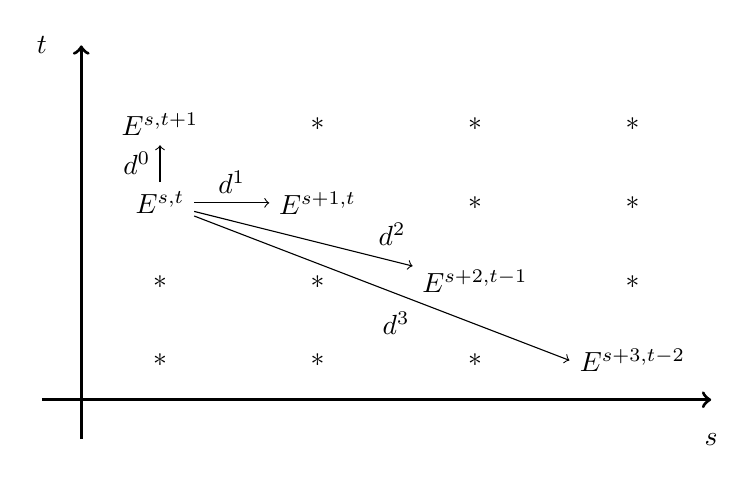
\begin{tikzpicture}
			\draw[very thick, ->] (-1.5, -0.5) -- (7,-0.5);
			\draw[very thick, ->] (-1,-1) -- (-1,4);
			\draw 
			(0,3) node(B){$E^{s,t+1}$} (2,3) node{$\ast$} (4,3) node{$\ast$} (6,3) node{$\ast$}
			(0,2) node(A){$E^{s,t}$} (2,2) node(C){$E^{s+1,t}$} (4,2) node{$\ast$} (6,2) node{$\ast$}
			(0,1) node{$\ast$} (2,1) node{$\ast$} (4,1) node(D){$E^{s+2,t-1}$} (6,1) node{$\ast$}
			(0,0) node{$\ast$} (2,0) node{$\ast$} (4,0) node{$\ast$} (6,0) node(E){$E^{s+3,t-2}$};
			\draw 
			(-1.5,4) node{$t$} (7,-1) node{$s$};
			
			\draw[->] (A) --node[anchor=east]{$d^{0}$} (B);
			\draw[->] (A) --node[anchor=south]{$d^{1}$} (C);
			\draw[->] (A) --node[anchor=south west, pos=0.8]{$d^{2}$} (D);
			\draw[->] (A) --node[anchor=north east, pos=0.6]{$d^{3}$} (5.2,0);
			
		\end{tikzpicture}
		\caption{I primi differenziali di bigrado $(r,1-r)$ in un bimodulo
		con notazione coomologica.}
    	\label{ss-differenziali}
	\end{figure}



\begin{oss}
	Un modulo bigraduato $E_{\bullet,\bullet}$ dà origine ad un complesso di catene
	\begin{equation*}
		K_{n} := \bigoplus_{s+t=n} E_{s,t}\,,
	\end{equation*}
	e in maniera duale, se il modulo ha la convenzione coomologica $E^{\bullet, \bullet}$,
	allora dà origine a un complesso di cocatene $K^{\bullet}$.
\end{oss}

Dato un modulo bigraduato $(E_{\bullet,\bullet},d)$, 
dato che $d^{2}=0$, possiamo calcolare la sua omologia $(p,q)$-esima 
come il quoziente
\begin{equation*}
	H_{p,q}(E_{\bullet,\bullet},d) := \dfrac{\ker\left( d : E_{p,q} \to E_{p-r,q+r-1} \right)}{\operatorname{im}\left( d: E_{p+r,q-r+1} \to E_{p,q} \right)}\,,
\end{equation*}
e la stessa cosa accade per la coomologia di $E^{\bullet,\bullet}$. 

\begin{df}
	Una \textbf{successione spettrale} di tipo \textbf{omologico}
	è una collezione di $R$-moduli differenziali bigraduati 
	$\Set{ \left(E^{r}_{\bullet,\bullet},d^{r}\right)}_{r \ge k}$,
	con $d^{r}$ di bigrado $(-r,r-1)$ tale che 
	\begin{equation*}
		E^{r+1}_{p,q} \simeq H_{p,q} \left( E_{\bullet,\bullet}^{r}, d^{r} \right)\,.
	\end{equation*}
	Analogamente, una \textbf{successione spettrale} di tipo \textbf{coomologico}
	è una collezione di $R$-moduli differenziali bigraduati 
	$\Set{ \left(E_{r}^{\bullet,\bullet},d_{r}\right)}_{r \ge k}$,
	con $d_{r}$ di bigrado $(r,-r+1)$ tale che 
	\begin{equation*}
		E_{r+1}^{p,q} \simeq H^{p,q} \left( E^{\bullet,\bullet}_{r}, d_{r} \right)\,.
	\end{equation*}
\end{df}

D'ora in avanti enunceremo definizioni e teoremi per uno solo dei due tipi
(per lo più il caso coomologico), ma è bene tenere a mente che
le costruzioni valgono in maniera analoga per entrambe le situazioni.

\begin{oss}
	Per definizione, la pagina $r$-esima $(E_{r}^{\bullet,\bullet},d_{r})$
	determina $E_{r+1}^{p,q}$, ma in generale
	\emph{non} determina il differenziale $d_{r+1}$ della pagina successiva.
\end{oss}

Una successione spettrale va pensata come una successione di pagine,
proprio come in un libro; in quanto tale, vorremmo conoscere
il suo comportamento ``alla fine'', ovvero studiare il suo \emph{limite}.
Per ogni $r \ge k$, indichiamo con $Z_{r}=\ker d_{r}$ i \textbf{cocicli} 
e con $B_{r}=\operatorname{im}d_{r}$ i \textbf{cobordi} del differenziale;
dato che $E_{r+1}=Z_{r}/B_{r}$, possiamo vedere il differenziale $(r+1)$-esimo
come un omomorfismo $d_{r+1} : Z_{r}/B_{r} \to Z_{r}/B_{r}$ e quindi 
considerare i suoi cocicli $Z_{r+1}$ come un (\emph{quoziente di un})
sottomodulo di $Z_{r}$ che contiene i cobordi $r$-esimi,
e lo stesso vale per $B_{r+1}$, quindi
\begin{equation*}
	B_{r} \subset B_{r+1} \subset Z_{r+1} \subset Z_{r}\,. 
\end{equation*}
Reiterando questo ragionamento per tutte le pagine, si ottiene la catena di inclusioni
\begin{equation*}
	B_{k} \subset B_{k+1} \subset B_{k+2} \subset \dots \subset Z_{k+2} \subset Z_{k+1} \subset Z_{k}\,.
\end{equation*}

\begin{df}
	Usando la convenzione sopra,
	poniamo $B_{\infty} := \cup_{i} B_{i}$ e $Z_{\infty} := \cap_{i} Z_{i}$.
	Definiamo il \textbf{limite della successione spettrale} come il quoziente
	$$E_{\infty} := Z_{\infty}/B_{\infty}\,.$$
\end{df}

Dalla definizione schietta è pressoché impossibile
calcolare il limite di una successione spettrale:
di solito speriamo che le cose vadano particolarmente bene
e quindi riuscire a aggirare questo problema di calcolo.
Introduciamo così una nozione di \emph{convergenza}.

\begin{df}
	Sia $H^{*}$ un $R$-modulo graduato.
	Una successione spettrale $\Set{(E_{r}^{\bullet,\bullet},d_{r})}_{r \ge k}$
	si dice \textbf{convergente a $H^{*}$} se esiste 
	una filtrazione %decrescente 
	$F^{\bullet}$ su $H^{*}$ tale che
	\begin{equation*}
		E_{\infty}^{p,q} \simeq E_{0}^{p}(H^{p+q})\,.
	\end{equation*}
\end{df}

\begin{oss}
	L'idea di \emph{convergenza} di una successione spettrale
	è che la \emph{digaonale} $p+q=n$ dell'elemento limite
	vada a ``approssimare'' il sottomodulo $H^{n}$
	tramite un modulo graduato associato.
\end{oss}

Sotto opportune ipotesi,
possiamo trovare delle situazioni dove il limite è più ``addomesticabile'',
ad esempio quando ogni bicomplesso $E^{\bullet,\bullet}_{r}$ vive nel primo quadrante,
cioè $E^{p,q}_{r} \ne 0$ solo per $p,q \ge 0$.
Allora i differenziali $d_{r}$ sono \emph{definitivamente nulli},
quindi la successione spettrale converge in un senso più forte:
si dice che la successione \textbf{stabilizza} se, per ogni $(p,q)$,
esiste un intero $r(p,q)$ tale che,
i differenziali $d_{r}^{p,q}=0$ e $d^{p-r,q+r-1}_{r}=0$ per ogni $r \ge r(p,q)$.
Da questo segue che $E_{r+1}^{p,q}=E_{r}^{p,q}$, da cui deduciamo che
se la successione in $(p,q)$ stabilizza, allora
\begin{equation*}
	E^{p,q}_{r} = E^{p,q}_{r+1} = E^{p,q}_{r+2} = \dots = E^{p,q}_{\infty}\,.
\end{equation*}

\begin{df}
	Diremo che una successione spettrale \textbf{collassa} alla pagina $N$
	se $d_{r}=0$ per ogni $r \ge N$.
\end{df}

\begin{df}
	Una filtrazione si dice \textbf{convergente} se $\cup_{s} F_{s}A = A$
	e $\cap_{s} F_{s}A = \{0\}$.
	Una filtrazione su un $R$-modulo graduato $A$ si dice 
	\begin{itemize}
		\item  \textbf{limitata dall'alto} se per ogni grado $t \in \Z$, 
		esiste un termine della filtrazione $s(t) \in \Z$ tale che $F_{s(t)}A_{t}=A_{t}$;
		\item  \textbf{limitata dal basso} se per ogni $t \in \Z$, esiste $u(t) \in \Z$
		tale che $F_{u(t)}A_{t} = 0$.
	\end{itemize}
\end{df}

%\begin{thm}
%	Un complesso di catene graduato e filtrato $(A,d,F)$ determina una successione spettrale
%	$\Set{(E_{\bullet,\bullet}^{r},d^{r})}$ tale che
%	$E_{s,t}^{1} = H_{s+t}(F_{s}A/F_{s-1}A)$ e il differenziale $d^{1}$ è
%	l'operatore di bordo della tripla $(F_{s}A,F_{s-1}A,F_{s-2})$.
%	Se la filtrazione $F_{\bullet}$ è convergente e limitata sia dal basso, sia dall'alto,
%	allora la successione spettrale stabilizza e converge al limite $E^{\infty}_{p,q}$
%	che è isomorfo al quoziente $F_{p}H_{p+q}(A)/F_{p-1}H_{p+q}(A)$.
%\end{thm}
%
%
%
%
%
%
%
%

\begin{ex}
	Prima di approfondire ulteriormente la teoria dietro alle successioni spettrali,
	possiamo cominciare a acquisire familiarità con queste tecniche dimostrando il
	seguente
	\begin{thm}[\textbf{Successione di Wang}]\label{wang}
		Sia $\Set{(E_{r}^{\bullet,\bullet},d_{r})}_{r \ge 2}$
		una successione spettrale nel primo quadrante, tale che
		per ogni $p \ne 0,n$ si abbia $E_{2}^{p,q} = 0$.
		Se la successione converge a $H^{*}$, allora esiste una successione esatta lunga
		\begin{equation*}
			\begin{tikzcd}
				\dots \ar[r]
				& H^{k} \ar[r]
				& E^{0,k}_{2} \ar[r, "d_{n}"]
				& E^{n,k-n+1}_{2} \ar[r]
				& H^{k+1} \ar[r]
				& \dots
			\end{tikzcd}
		\end{equation*}
		\begin{proof}
			La pagina $E_{2}^{\bullet,\bullet}$ è concentrata
			nella $0$-esima e nella $n$-esima colonna, come mostrato in
			\hyperref[wang-e2]{Figura~\ref{wang-e2}}.
			Si deduce immediatamente che i differenziali della successione
			sono tutti nulli, fatta eccezione di $d_{n}$.
			
	\begin{figure}
		\centering
		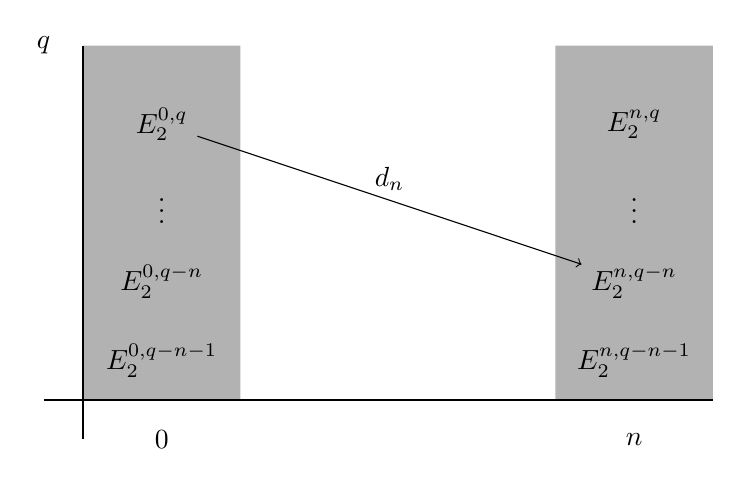
\begin{tikzpicture}
			\fill[opacity=.3] (-1,-0.5) -- (1, -0.5) -- (1,4) -- (-1,4) -- (-1,-0.5);
			\fill[opacity=.3] (5,-0.5) -- (7, -0.5) -- (7,4) -- (5,4) -- (5,-0.5);
			\draw[thick] (-1.5, -0.5) -- (7,-0.5) (-1,-1) -- (-1,4);
			\draw 
			(0,3) node(A){$E_{2}^{0,q}$} (6,3) node{$E_{2}^{n,q}$}
			(0,2) node{$\vdots$}  (6,2) node{$\vdots$}
			(0,1) node{$E_{2}^{0,q-n}$} (6,1) node(B){$E_{2}^{n,q-n}$}
			(0,0) node{$E_{2}^{0,q-n-1}$} (6,0) node{$E_{2}^{n,q-n-1}$};
			\draw 
			(-1.5,4) node{$q$} (0,-1) node{$0$} (6,-1) node{$n$};
			\draw[->] (A) --node[anchor=south]{$d_{n}$} (B);
		\end{tikzpicture}
		\caption{Pagina $E^{\bullet,\bullet}_{2}$ come nelle ipotesi del \hyperref[wang]{Teorema~\ref{wang}}.}
    	\label{wang-e2}
	\end{figure}
			
			La successione spettrale collassa alla pagina $n+1$
			e si può dedurre che il limite è
			\begin{equation*}
				E^{0,q}_{\infty} \simeq 
				\ker \left( d_{n} : E^{0,q}_{2} \to E^{n,q-n+1}_{2} \right)\,,
				\quad 
				E^{n,q}_{\infty} \simeq 
				\operatorname{coker}\left( d_{n} : E^{0,n+q-1}_{2} \to E^{n,q}_{2} \right)\,,
			\end{equation*}
			quindi per ogni $q \in \Z$ abbiamo la successione esatta
			\begin{equation}\label{wang-A}
				\begin{tikzcd}
					\cat{0} \ar[r]
					& E^{0,q}_{\infty} \ar[r]
					& E^{0,q}_{2} \ar[r, "d_{n}"]
					& E^{n,q-n+1}_{2} \ar[r]
					& E^{n,q-n+1}_{\infty} \ar[r]
					& \cat{0} \,.
				\end{tikzcd}\tag{A}
			\end{equation}
			D'altra parte, l'ipotesi che $E^{\bullet,\bullet}_{r}$ converge 
			a $H^{*}$ ci permette di dedurre informazioni sulla
			filtrazione $F$ che c'è su questo modulo: infatti,
			dato che per $p \ne 0,n$ si ha
			\begin{equation*}
				\cat{0} \simeq E^{p,q}_{\infty} \simeq 
				\frac{F^{p}H^{p+q}}{F^{p+1}H^{p+q}}\,,
			\end{equation*}
			deduciamo che la filtrazione su $H^{*}$ ha al più due termini:
			per ogni $k \in \Z$, studiando
			gli elementi della forma $E^{p,k-p}_{\infty}$ si vede che
			\begin{equation*}
				H^{k} = F^{0}H^{k} \supset F^{1}H^{k} = F^{2}H^{k} = \dots
				= F^{n}H^{k} \supset F^{n+1}H^{k} = \cat{0}\,.
			\end{equation*}
			Da questo si deduce che 
			$E^{0,k}_{\infty} \simeq F^{0}H^{k}/F^{n}H^{k} \simeq H^{k}/E^{n,k-n}_{\infty}$
			e quindi esiste una successione esatta corta
			\begin{equation}\label{wang-B}
				\begin{tikzcd}
					\cat{0} \ar[r]
					& E^{n,k-n}_{\infty} \ar[r]
					& H^{k} \ar[r]
					& E^{0,k}_{\infty} \ar[r]
					& \cat{0} \,.
				\end{tikzcd}\tag{B}
			\end{equation}
			``Incollando'' le \eqref{wang-A} con le \eqref{wang-B},
			otteniamo la \textbf{successione di Wang}, 
			tratteggiata nel diagramma sottostante:
			\begin{equation*}
				\begin{tikzcd}
					& \cat{0} \ar[d] & & & & \\
					\dots \ar[r] \ar[dr, dashed] & E^{n,k-n}_{\infty} \ar[d] \ar[r]& \cat{0} & & & \\
					& H^{k} \ar[d] \ar[dr, dashed] & & & \cat{0} \ar[d] & \\
					\cat{0} \ar[r] & E^{0,k}_{\infty} \ar[r] \ar[d] & E^{0,k}_{2} \ar[r, "d_{n}", dashed]
					& E^{n,k-n+1}_{2} \ar[r] \ar[dr, dashed] & E^{n,q-n+1}_{\infty} \ar[r] \ar[d] & \cat{0} \\
					& \cat{0} & & & H^{k+1} \ar[d] \ar[dr, dashed] & \\
					& & & \cat{0} \ar[r] & E^{0,k+1}_{\infty} \ar[d] \ar[r] & \dots \\
					& & & & \cat{0} & \,.
				\end{tikzcd}
			\end{equation*}\qedhere
		\end{proof}
	\end{thm}
\end{ex}
































